User can define a cube(3D),rectangular cube(3D),plane(2D),line(1D) or a point with this primitive by defining its lower-left-bottom and upper-right-top edge.

\begin{FontNameFunct}{AddBox()}
\end{FontNameFunct} 

\begin{FontDescr}{Purpose:}
Add a box to \matv{CSX}\phantomsection\label{CSX} with predefined property in either cartesian- or cylindrical- coordinate. The name of property and primitive must match.  
\end{FontDescr}

\begin{FontDescr}{Syntax:}
\begin{lstlisting} 
 CSX = AddBox(CSX, propName, prio, start, stop, varargin)
\end{lstlisting}
\end{FontDescr}

\begin{FontDescr}{Description:}

\begin{FontPara}{propName} \phantomsection \label{prim_Name}
Primitive Name which must be the same with that mentioned in the \texttt{Add<...property...>}. Refer to \hyperref[subsection_gprop_setup]{subsection 4.1.1}.
\end{FontPara}

\begin{FontPara}{start}
Start coordinate of a box.(vector)
\end{FontPara}

\begin{FontPara}{stop}
Stop coordinate of a box.(vector)
\end{FontPara}

\end{FontDescr}

\begin{FontDescr}{Optional Arguments:} \phantomsection \label{primtransform}
\begin{FontPara}{'Transform'}
Transformation of a primitive in 3D material/metal discretisation.
\begin{itemize}
\item\textcolor{varcol}{'Scale'}: scale the model with scale factor.\\ For example,'1,1,2': the z-dimension is scaled with 2. 

\item\textcolor{varcol}{'Rotate$\_$X'}:  Rotate the structure around x-axis.\\ For example, pi/4: structure will be rotated $45^{0}$. \\'Rotate$\_$Y' and 'Rotate$\_$Z' are available too.  

\item\textcolor{varcol}{'Translate'}: Translate the structure with defined distance.\\For example,'0,0,100': model will be z-direction shifted to 100 drawing unit.
\end{itemize}
\end{FontPara}
\end{FontDescr}

\begin{FontDescr}{Examples:}

\begin{lstlisting}
 CSX=InitCSX('CoordSystem',0);
 CSX = AddMetal(CSX,'metal'); 
 CSX = AddBox(CSX,'metal',10,[0 0 -100],[100 100 0]);
\end{lstlisting} 
A metal box has been defined in Cartesian coordinate and has size 100x100x100 in drawing unit.

\begin{lstlisting}
CSX=InitCSX('CoordSystem',0);
CSX = AddMetal(CSX,'metal'); 
CSX = AddBox(CSX,'metal',10,[0 0 -100],[100 100 0],
'Transform', {'Rotate_Z', pi/4});  
\end{lstlisting}  
The box is then rotated $45^{0}$ around z-axis.   

\begin{lstlisting}
 CSX=InitCSX('CoordSystem',0);
 CSX = AddMetal(CSX,'metal2'); 
 CSX = AddBox(CSX,'metal2',10,[0 0 0],[100 100 0],
 'Transform',{'Translate', '100,0,0','Scale','1/10,1,1'});
\end{lstlisting} 
This creates a strip of size 10x100 on z=0. The strip is originally created at origin with size 100x100. It is then translated to x=100 and scaled with factor 1/100 on x-dimension. The start point of strip has been transformed into x=10,y=0 and end point x=20,y=100. The translation distance has been also scaled! Refer to Fig.\ref{fig:primBoxtransform}((a),(b),(c)).

\begin{lstlisting}
 CSX=InitCSX('CoordSystem',0);
 CSX = AddMetal(CSX,'metal2'); 
 CSX = AddBox(CSX,'metal2',10,[0 0 0],[100 100 0],
 'Transform',{'Scale','1/10,1,1','Translate', '100,0,0'});
\end{lstlisting}

If scalation is done before translation, the strip will be of the same size but at different start and end point. Refer to Fig. \ref{fig:primBoxtransform}((a),(d),(e)).     

\begin{figure}[h!]
\centering
\includegraphics[width=0.85\textwidth]{svg/primBox_transform.pdf}
\caption{Transformation of strip on z-plane}
\label{fig:primBoxtransform}
\end{figure}

    
The following example will describe the box definition in cylindrical coordinate: 

\begin{lstlisting} 
 CSX=InitCSX('CoordSystem',1);
 CSX = AddMetal(CSX,'metal'); 
 CSX = AddBox(CSX,'metal',10,[-100 0 0],[100 2*pi 0]);
\end{lstlisting}
This example creates a circle of radius=100 with \texttt{AddBox} function. User can also use \texttt{AddCylinder}(section \ref{cylinder}) function to build this circle. 

\begin{lstlisting} 
 CSX=InitCSX('CoordSystem',1);
 radius=100;
 mesh_factor=[1 1/radius 1];
 CSX = AddMetal(CSX,'metal'); 
 CSX = AddBox(CSX,'metal',10,[0 0 -100].* mesh_factor,[100 100 0].* mesh_factor);
\end{lstlisting}

The metal box Fig.\ref{fig:primBoxtransform}(a) has been transformed($\Rightarrow $) into a sector of a circle with radius=100(Fig.\ref{fig:box in cyl}(a)). The dimension of a box: 

\begin{itemize}
\item x=0 $\rightarrow$ 100    $\Rightarrow $   r=0 $\rightarrow$ 100

\item y=0$\rightarrow$ 100     $\Rightarrow $   a=0 $\rightarrow$ 100/radius(=1 radian)

\item z=-100$\rightarrow$ 0   $\Rightarrow $   z=-100 $\rightarrow$ 0
\end{itemize}            

\begin{lstlisting} 
 CSX=InitCSX('CoordSystem',1);
 radius=100;
 mesh_factor=[1 1/radius 1];
 CSX = AddMetal(CSX,'metal'); 
 CSX = AddBox(CSX,'metal',10,[100 0 0].* mesh_factor,[110 100 0].* mesh_factor);
\end{lstlisting}

The strip shown in Fig.\ref{fig:primBoxtransform}(e) has been bended as it is  defined in Cylinder coordinate system(Fig.\ref{fig:box in cyl}(b)).   

\begin{itemize}
\item x=100 $\rightarrow$ 110    $\Rightarrow $   r=100 $\rightarrow$ 110

\item y=0$\rightarrow$ 100     $\Rightarrow $   a=0 $\rightarrow$ 100/radius(=1 radian)

\item z=0$\rightarrow$ 0   $\Rightarrow $   z=0 $\rightarrow$ 0
\end{itemize}  

\begin{figure}[hbt]

\centering
\subfloat[Sector of a circle]
{\includegraphics[width=0.4\textwidth]{svg/box_cylinderco.pdf}}
\subfloat[Bended strip]{\includegraphics[width=0.41\textwidth]{svg/bended_strip.pdf}}
\caption{Top view of the transformed box(a) and strip(b).}
\label{fig:box in cyl}
\end{figure}

\end{FontDescr}


